%-------------------------------------------------------------------

\thispagestyle{empty}
\begin{center}
\vspace*{1.4in}
{\LARGE  {\bf UNIVERSITY OF MICHIGAN   \vspace*{0.7in} \\   
   Department of Nuclear Engineering \\ and Radiological Sciences
      \vspace*{0.7in} \\

   APPLIED MATHEMATICS FOR ENGINEERING PHYSICS \vspace*{0.7in} \\
   Brian Kiedrowski }} \\
    \vspace{1cm} {\bf \today}
\end{center}
\pagebreak

%-------------------------------------------------------------------

\setcounter{page}{1}
\setcounter{chapter}{0}
\pagenumbering{roman}

% \vspace*{3.0in}
 \begin{center}
 \copyright \; {\large Brian Christopher Kiedrowski \\
 --------------------------------------- \\
 All Rights Reserved \\
 2024 }
 \end{center}
 
 \vspace*{3em}
\noindent \small This textbook may be freely used for educational purposes, either personal or to support teaching. If used as a textbook for a course, I request a courtesy email indicating as such. This allows for me to measure the impact of the works. \\

\noindent  This textbook is provided on an ``AS IS'' BASIS, WITHOUT WARRANTIES OR CONDITIONS OF ANY KIND, either express or implied, including, without limitation, any warranties or conditions of TITLE, NON-INFRINGEMENT, MERCHANTABILITY, or FITNESS FOR A PARTICULAR PURPOSE. You are solely responsible for determining the appropriateness of using or redistributing the Work and assume any associated risks. \\

\noindent LaTeX source for this textbook is available at \\ \url{https://github.com/bckiedrowski/textbooks}. \\

\noindent The author (Brian Kiedrowski) retains rights to all parts of the source code and finished products. Derivative works based on these texts are permitted subject to the following restrictions:
\begin{enumerate}
  \item Brian Kiedrowski shall retain primary/first authorship followed by those authoring the derivative work.
  \item The authorship in the lower-left corner of each page shall be present in all derivative works and shall include B.C. Kiedrowski as first author.
  \item Neither the originals nor derivative works shall be commercialized, sold for profit, nor submitted to a publisher without the consent of Brian Kiedrowski.
  \item All derivative works must include the text of the copyright page. Authors of derivative works may provide additional terms and conditions. In the event that there is a conflict, the terms and conditions in the original document shall take precedence.
\end{enumerate}

\noindent Contact information: \texttt{bckiedro@umich.edu}.
\normalsize

%-------------------------------------------------------------------
%
%\vspace*{2.4in}
%These notes include material from the following sources:
%
%\begin{enumerate}
%  \item A.M. Weinberg and E.P. Wigner, {\em The Physical Theory of
%        Neutron Chain Reactors}, University of Chicago Press, Chicago 
%        (1958).
%  \item G.I. Bell and S. Glasstone, {\em Nuclear Reactor Theory}, Van
%        Nostrand Reinhold, New York (1970)*
%  \item J.J. Duderstadt and L.J. Hamilton, {\em Nuclear Reactor
%        Analysis}, Wiley, New York (1976).*
%  \item R.A. Rydin, {\em Nuclear Reactor Theory and Design}, second
%        edition (1993).
%  \item W.M. Stacey, {\em Nuclear Reactor Physics}, Wiley, New York
%        (2001).
%\end{enumerate}
%
%\vspace{10pt} 
%* These books are recommended as supplementary texts. \\

%The authors wish to thank the following individuals: Jipu Wang, who provided an extraordinary number of corrections to these notes; Matthew Gonzales, who provided information regarding analytic solutions to the heavy gas model in Sec.~\ref{Sec:Thermal_HeavyGasAnalyticSolution}; and Andrew Pavlou, who provided numerical $S(\alpha,\beta)$ data used in Sec.~\ref{Sec:Thermal_BoundScatteringPhysics_Solids_Graphite}.

\tableofcontents

\clearpage
\pagenumbering{arabic}
\setcounter{page}{1}
\chapter{Introduction}

This textbook is designed to review and add engineering context and relevance for the undergraduate math sequence at the University of Michigan with a specific focus on the discipline of nuclear engineering. Given the breadth of the nuclear field, the contents herein should also be applicable to other engineering disciplines as well. Specifically, this text contains mathematical techniques relevant to mechanics, fluids and heat transfer, electromagnetism, quantum mechanics, in addition to topics such as neutron diffusion and nuclear criticality.

For University of Michigan students in Nuclear Engineering and Radiological Sciences, the field makes heavy use of mathematics and computing and NERS 320 is meant to provide students a solid mathematical foundation relevant to the advanced undergraduate coursework and beyond, whether that be a career in industry, graduate school, etc. This course assumes that students have completed the standard mathematics sequence at the University of Michigan. In particular, this course relies heavily on the material in Calculus~III, multivariate calculus, and Calculus~IV, ordinary differential equations. 

The course has five units: linear algebra, systems of ordinary differential equations, vector calculus, partial differential equations, and probability. Each unit is a course unto itself; as such, this text can only superficially cover these topics and is not a substitute for the aforementioned mathematics courses or other math courses that can cover these topics in greater depth. 

\section{Mathematical Models in Engineering}

Mathematics is the language that scientists and engineers use to describe the workings of the universe. It offers a consistent framework and set of rules by which we can explain and manipulate the forces of nature for the benefit of humanity and the planet. A common goal of science and engineering is to take a complicated set of phenomena and construct a mathematical model that we hope is relevant and has high enough fidelity for its purpose. In constructing such as model, it is important to realize that all such models are limited by either concerns of practicality of solving the equations or from ignorance about the underlying processes. For this it is the responsibility of the scientist or engineer to ensure that the mathematical model, the model parameters, and the techniques to solve the equations in the model are adequate for the task at hand.

Some examples of mathematical models we encounter in the nuclear engineering discipline are as follows. The first of these are the Bateman equations that describe the production and decay of a population of isotopes:
\begin{align}
  \frac{dN_i}{dt} = -\lambda_i N_i(t) + \sum_j f_{ij} \lambda_j N_j(t) + Q_i(N_1(t),N_2(t),\cdots,t).
\end{align}
This is a coupled set of equations and are important in the fields of health physics, the design of nuclear fission and fusion reactors, and the management of radioactive and nuclear materials. Note that the production term $Q$ may be a function of the isotopes in the system itself and is an important consideration in nuclear fission reactors where the isotope mixture impacts the neutron radiation field that produces the isotopes.

Another important equation for NERS is the heat equation, which describes the flow of thermal energy through a system and obtains an unknown temperature field $T(x,y,z,t) = T(\pos,t)$ that varies in space and time:
\begin{align}
  \rho c_p \frac{ \partial T }{ \partial t } - \nabla \cdot k(\pos,T) \nabla T(\pos,t) = q(\pos,t).
\end{align}
This partial differential equation is important because nuclear reactions are often used as a heat source for various applications such as nuclear fission or fusion reactors, radioisotope thermoelectric generators, and as a consequence of energy deposition by fields of radiation.

A related and more complicated equation is the one that describes the flow of fluids with an unknown velocity field $\mathbf{u}(\pos,t)$. These are the Navier-Stokes equations for compressible flow:
\begin{align}
  \dho{}{t}(\rho \mathbf{u}) + \nabla \cdot ( \rho \mathbf{u} \otimes \mathbf{u} ) = -\nabla p + \mu \nabla^2 \mathbf{u} + \frac{1}{3} \mu \nabla ( \nabla \cdot \mathbf{u} ) + \rho \mathbf{g}.
\end{align}
This equation is inherently nonlinear and gives rise to turbulence, perhaps one of the most difficult phenomena to model in physics. The relevance of this equation is that it is the one that governs fluid motion, which is vital in heat removal for nuclear systems. It is also one of the equations that may be used for the flow of plasmas, which is vital to understanding systems involving nuclear fusion.

Nuclear fusion systems require extreme temperatures that require an understanding of the physics of plasmas or ionized gasses. In plasmas and fusion systems, the behavior of electromagnetic fields is of primary concern. Additionally, the equations of electromagnetism arises in the study of radiation detection. The relevant equations are Maxwell's equations, which can be written in either differential or integral form. The differential form of these are:
\begin{subequations}
\begin{align}
  \nabla \cdot \mathbf{E} &= \frac{\rho}{\epsilon_0}, \text{ (Gauss' law)} \\
  \nabla \cdot \mathbf{B} &= 0, \\
  \nabla \times \mathbf{E} &= -\dho{\mathbf{B}}{t}, \text{ (Faraday's law)} \\
  \nabla \times \mathbf{B} &= \mu_0 \left( \mathbf{J} + \epsilon_0 \dho{\mathbf{E}}{t} \right), \text{ (Ampere's law)}.
\end{align}
\end{subequations}
Maxwell's equations involve a heavy amount of vector calculus with the unknowns being the components of the electric field $\mathbf{E}$ and magnetic field $\mathbf{B}$. Also, they are often combined with the fluids equations through the external force term $\mathbf{g}$ in plasma physics applications.

The last of this list is the equation describing the evolution of a radiation field. This is done with the linear Boltzmann equation that describes the position, direction, kinetic energy, and time (7 dimensions) of the radiation field:
\begin{align}
  &\frac{1}{v} \dho{\psi}{t} + \dir \cdot \nabla \psi(\pos,\dir,E,t) + \Sigma_t(E) \psi(\pos,\dir,E,t) \nonumber \\
  &= \iint \Sigma_s(E' \rightarrow E, \dir' \cdot \dir )  \psi(\pos,\dir',E',t) d\Omega' dE' + Q(\pos,\dir,E,t).
\end{align}
Of note is that this is an integro-differential equation in that the process of scattering (radiation changing direction and energy in collisions) is an integral over the incident directions and energies. This coupled with the dimensionality of the problem presents its own set of challenges that are largely unique to nuclear engineering.

By no means is this list comprehensive; rather, it is meant to illustrate the complexity and mathematical richness of the physics encountered in NERS and motivate the need for the mathematical content in this text.

\section{Computational Physics}

In the ideal word, we would encounter a set of equations describing physical phenomena (usually partial differential equations) and we would go about obtaining analytical solutions. Unfortunately, this is usually only possible in a limited set of cases that are usually too simplistic for practical engineering. Therefore, we invariably must take those equations in our mathematical model and apply techniques to approximate them as a simpler set of equations that we are capable of solving, usually only numerically. These equations are then often implemented in some computer software that we use to obtain numerical results.

This is the essence of using mathematics in engineering and will be a common theme of the course. Throughout this course, we will cover some of the basic considerations with approximating the complex models encountered in NERS with simpler ones. Before going into detail, it is important to cover two vital topics in scientific computing called verification and validation. In short, it is the responsibility of the engineer to ensure their mathematical models are being solved correctly and that they are applicable to the engineering problem. Failure to do suitable verification and validation can lead to erroneous results that can lead to flawed design decisions being made with potentially life threatening impacts. For this reason, ensuring correctness and suitability of mathematical models is also an important theme of this course.

\subsection{Verification}

An approximate set of equations are obtained from a more general mathematical model and these approximate equations are then solved using some computer code. For a given engineering design application, it is important to certify that the software is actually solving its equations correctly and as intended. Much of the responsibility for this falls onto the software developer; however, it is important for the end user engineer to ensure that the relevant portions of the software have been adequately verified.

Some examples of verification methods are as follows:
\begin{itemize}
  \item {\bf Unit testing} checks individual operations and functions within the software to ensure that each small unit of the code is doing the intended operation. While this strategy is important for catching many errors in the software, and vital to the development process, it is impractical to apply unit testing in a way that stresses all possible combinations of cases throughout a large simulation code. Usually this is done by the software developer and is noted by the end user in deciding the quality of the software.
  \item {\bf Benchmark comparisons} check the ability of the code to calculate results of reference solutions. The ``gold standard'' for this are analytical benchmarks, which involve comparing simulation results against solutions of the underlying differential equation(s); these solutions tend to be few and only for very simple cases, but can be revealing of deficiencies in the software. The next best thing are numerical benchmarks that have been obtained using alternative approaches to solving the problem that themselves may be too complicated to be practical except for benchmarking. Often software developers will do some of this and, where relevant to the specific problem, should be noted. In cases where this has not been performed for the application, it may be advisable to search the literature for analytical or numerical benchmarks or devise some that have some of the mathematical features of the application, but are simple enough to permit a solution.
  \item {\bf Code comparisons}, as the name implies, checks the solution from a particular software to another code that has hopefully been vetted. Ideally, the other code would use a different method to solve the same problem. When possible, it is good to occasionally double check the preferred design tool in an organization with another to provide confidence that the design calculations are being performed correctly. Usually, this is done exclusively by the end-user engineer and not the developers of the software.
\end{itemize}

Another consideration related to verification is ensuring the code is being used appropriately. Most methods involve approximating some differential equation in some manner; the most common of these involves transforming the differential equations into a set of linear equations described by a spatial mesh. A finer mesh preserves more of the mathematics of the initial equations, but at the expense of computational resources (memory and computational time). Many engineering calculations involve, for example, a mesh sensitivity study to ensure that the spatial grid is sufficiently resolved to retain an acceptable amount of fidelity in the model.

\subsection{Validation}

Validation is the process by determining whether the underlying mathematical models and the associated physical data (e.g., equation of state, physical properties, nuclear cross sections) are sufficiently accurate for the engineering application. This differs from verification in that it checks only that the mathematical equations are being solved correctly, not that the mathematical model itself is suitable. (It is possible, albeit very undesirable, for a code to solve equations incorrectly, but be ``good enough'' for the engineering design.)

The process of validation often involves comparing the results obtained from a code with numerical measurements of analogous quantities in scenarios ranging from small-scale laboratory experiments looking at one physical phenomenon, to prototypes that are simplified versions of the system, up to a full system in real-world operating conditions.  From these comparisons, a quantitative assessment of how predictive the code is with reality can be made. Additionally, validation exercises are often used to quantify the bias. For example, if a particular calculation tends to predict a mechanical stress that is 5-10\% lower than measurement for a given system, then this can be accounted for in the design process and mathematical models are calibrated accordingly. Many organizations will devote resources to performing experiments whose sole purpose is to test and calibrate computational models. Indeed, much of the historical nuclear engineering design work relied on comparing prototypes and then operating reactors to calculations and then calibrating results accordingly, and this is still ongoing today, albeit at a smaller scale.

As part of the engineer using software for design and analysis, it is important to be aware of what experiments have been performed relevant or similar systems that can be used to test the predictive capability of the computational design models and to perform those comparisons. Depending on the nature of the work, there may need to be conversations between the analysts and the experimenters to develop suitable experiments to test the models.

An example in the nuclear engineering field is the area of criticality safety, which concerns itself with the safe handling of fissionable materials in industrial processes to avoid the formation of a critical mass of nuclear material. For this work, software that simulates the neutron radiation throughout the systems of interest are employed to estimate the nuclear criticality or effective multiplication of the system. Unfortunately, the nuclear properties are not known well enough to give perfect agreement with reality, so criticality safety engineers perform validation studies by looking for benchmark experiments that are similar to the application, testing the radiation transport solver on those, and quantifying how well or poorly the code predicts the experiments. These results are analyzed statistically and margins or safety factors are put into the design process to ensure subcriticality.

In short, validation of software is the responsibility of the end-user engineer performing the analysis. While software developers may perform some of their own validation on a wide set of systems, they cannot be familiar with and test every possible application. And even if they could, it is still up to the engineer to understand how well (or poorly) the mathematical models, software, and material data perform together on the application to build in appropriate safety factors.

\subsection{Example: Radioactive Decay}

To illustrate the difference between the concepts of verification and validation, consider the simple case of radioactive decay. This follows the simple differential equation
\begin{align}
  \frac{dN}{dt} = -\lambda N(t), \quad N(0) = N_0 .
\end{align}
While this has a simple solution of an exponential,
\begin{align}
  N(t) = N_0 e^{-\lambda t} ,
\end{align}
numerical integration techniques can be applied to approximate the solution. (It is foolish to apply numerical techniques to such a simple case, but such techniques quickly become necessary as problems become too difficult to solve analytically.) The simplest numerical integration technique is called Forward Euler (see Sec.~\ref{Sec:ode_numericalTechniques} for details) and involves taking a finite time step $\Delta t$. If implemented correctly, the approximate solution from forward Euler should approach the analytic solution as $\Delta t$ becomes small. A verification exercise checks that this is indeed the case.

\begin{figure}[htp!]
\begin{center}
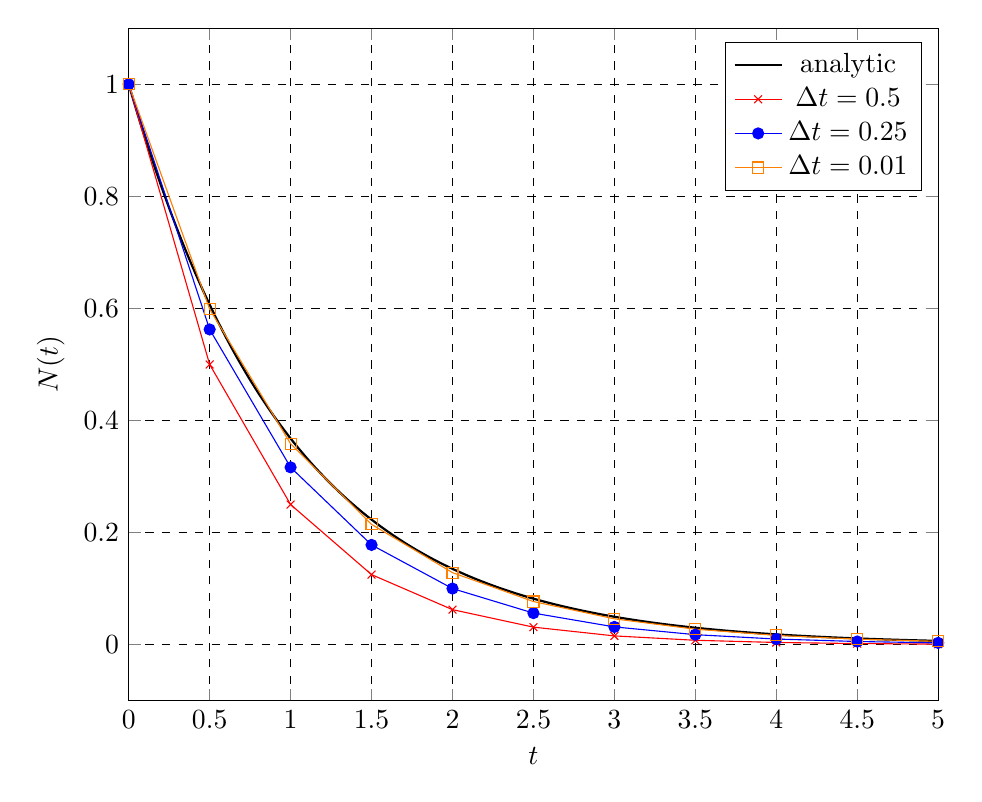
\begin{tikzpicture} \begin{axis}
[scale=1.5,
 xmin=0,    xmax=5,
 ymin=-0.1, ymax=1.1,
 grid=major, 
 major grid style={color=black,line width=0.2pt, dashed},
 xlabel=$t$,
 ylabel=$N(t)$,
]
\addplot[
   black,
   domain=0:5,
   samples=201,
   line width=0.8pt
]
{exp(-x)};
\addlegendentry{analytic}

\addplot[color=red,mark=x] coordinates {
 ( 0 , 1 ) 
 ( 0.5 , 0.5 ) 
 ( 1 , 0.25 ) 
 ( 1.5 , 0.125 ) 
 ( 2 , 0.0625 ) 
 ( 2.5 , 0.03125 ) 
 ( 3 , 0.015625 ) 
 ( 3.5 , 0.0078125 ) 
 ( 4 , 0.00390625 ) 
 ( 4.5 , 0.00195312 ) 
 ( 5 , 0.000976562 ) 
};
\addlegendentry{$\Delta t = 0.5$}
\addplot[color=blue,mark=*] coordinates {
 ( 0 , 1 ) 
 ( 0.5 , 0.5625 ) 
 ( 1 , 0.316406 ) 
 ( 1.5 , 0.177979 ) 
 ( 2 , 0.100113 ) 
 ( 2.5 , 0.0563135 ) 
 ( 3 , 0.0316764 ) 
 ( 3.5 , 0.0178179 ) 
 ( 4 , 0.0100226 ) 
 ( 4.5 , 0.00563771 ) 
 ( 5 , 0.00317121 ) 
};
\addlegendentry{$\Delta t = 0.25$}
\addplot[color=orange,mark=square] coordinates {
 ( 0 , 1 ) 
 ( 0.5 , 0.598737 ) 
 ( 1 , 0.358486 ) 
 ( 1.5 , 0.214639 ) 
 ( 2 , 0.128512 ) 
 ( 2.5 , 0.076945 ) 
 ( 3 , 0.0460698 ) 
 ( 3.5 , 0.0275837 ) 
 ( 4 , 0.0165154 ) 
 ( 4.5 , 0.00988836 ) 
 ( 5 , 0.00592053 ) 
};
\addlegendentry{$\Delta t = 0.01$}
\end{axis}
\end{tikzpicture}
\caption{Verification exercise for simple radioactive decay.}
 \label{Fig:intro_radioactiveDecayVerification}
\end{center}
\end{figure}

As a verification exercise, let $\lambda = 1$ and see how well the approximate numerical solution matches the analytic exponential solution in this case. This comparison is shown in Fig.~\ref{Fig:intro_radioactiveDecayVerification}. The dark solid line gives the analytic solution and dots (interpolated with lines for clarity) give points from the numerical solution for different time step sizes. Based on this result, one can say that the forward Euler method is correctly approximating the right equation and exhibits the expected limiting behavior.

\begin{figure}[htp!]
\begin{center}
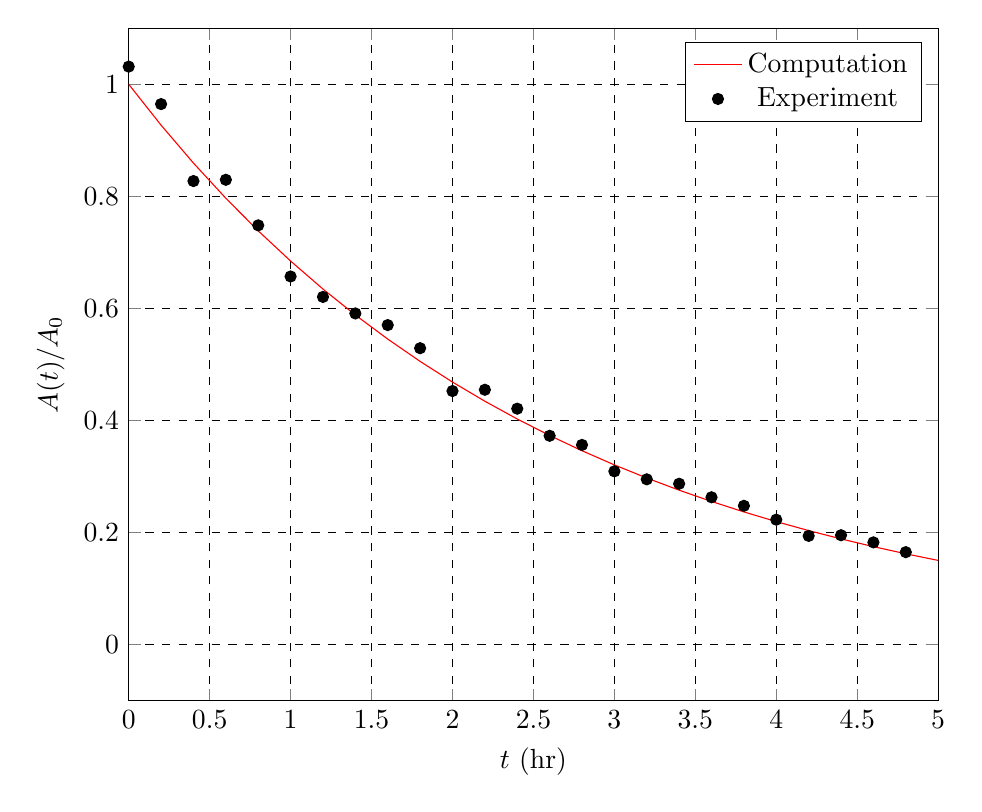
\begin{tikzpicture} \begin{axis}
[scale=1.5,
 xmin=0,    xmax=5,
 ymin=-0.1, ymax=1.1,
 grid=major, 
 major grid style={color=black,line width=0.2pt, dashed},
 xlabel=$t$ (hr),
 ylabel=$A(t)/A_0$,
]
%\addplot[
%   black,
%   domain=0:5,
%   samples=201,
%   line width=0.8pt
%]
%{exp(-x)};
%\addlegendentry{analytic}

\addplot[color=red] coordinates {
 ( 0 , 1 ) 
 ( 0.2 , 0.927 ) 
 ( 0.4 , 0.859329 ) 
 ( 0.6 , 0.796599 ) 
 ( 0.8 , 0.738447 ) 
 ( 1 , 0.684541 ) 
 ( 1.2 , 0.634569 ) 
 ( 1.4 , 0.588246 ) 
 ( 1.6 , 0.545304 ) 
 ( 1.8 , 0.505497 ) 
 ( 2 , 0.468596 ) 
 ( 2.2 , 0.434389 ) 
 ( 2.4 , 0.402678 ) 
 ( 2.6 , 0.373283 ) 
 ( 2.8 , 0.346033 ) 
 ( 3 , 0.320773 ) 
 ( 3.2 , 0.297357 ) 
 ( 3.4 , 0.27565 ) 
 ( 3.6 , 0.255527 ) 
 ( 3.8 , 0.236874 ) 
 ( 4 , 0.219582 ) 
 ( 4.2 , 0.203553 ) 
 ( 4.4 , 0.188693 ) 
 ( 4.6 , 0.174919 ) 
 ( 4.8 , 0.16215 ) 
 ( 5 , 0.150313 ) 
};
\addlegendentry{Computation}
\addplot[mark=*, only marks] coordinates {
 ( 0 , 1.03147 ) 
 ( 0.2 , 0.964619 ) 
 ( 0.4 , 0.827278 ) 
 ( 0.6 , 0.829532 ) 
 ( 0.8 , 0.748225 ) 
 ( 1 , 0.656995 ) 
 ( 1.2 , 0.620519 ) 
 ( 1.4 , 0.59101 ) 
 ( 1.6 , 0.570259 ) 
 ( 1.8 , 0.529004 ) 
 ( 2 , 0.452558 ) 
 ( 2.2 , 0.454838 ) 
 ( 2.4 , 0.421095 ) 
 ( 2.6 , 0.372744 ) 
 ( 2.8 , 0.356431 ) 
 ( 3 , 0.309292 ) 
 ( 3.2 , 0.295037 ) 
 ( 3.4 , 0.287116 ) 
 ( 3.6 , 0.263001 ) 
 ( 3.8 , 0.247765 ) 
 ( 4 , 0.223008 ) 
 ( 4.2 , 0.194108 ) 
 ( 4.4 , 0.195287 ) 
 ( 4.6 , 0.182516 ) 
 ( 4.8 , 0.165054 ) 
};
\addlegendentry{Experiment}
\end{axis}
\end{tikzpicture}
\caption{Validation of exponential decay model for $^{18}$F.}
 \label{Fig:intro_radioactiveDecayValidation_18F}
\end{center}
\end{figure}

Validation checks that the model is appropriate for the problem being analyzed and often involves using experimental data. For the purposes here, fictitious experimental data of radioactive detection counts are used. (This is generated for the plot by using the analytic solution and applying a random offset to each point to simulate the effect.) First, consider the isotope $^{18}$F, which is used in positron emission tomography, a medical diagnostic. $^{18}$F has a half life of 1.82~hr or a decay constant of $\lambda = 0.379$~hr$^{-1}$. The comparison of the activity computation versus the ``experimental'' data is given in Fig.~\ref{Fig:intro_radioactiveDecayValidation_18F}. While there is some variation because of the noise in the data (that would arise from measurement uncertainties because of a finite counting time), the computation appears to adequately represent the experimental data trends.

\begin{figure}[htp!]
\begin{center}
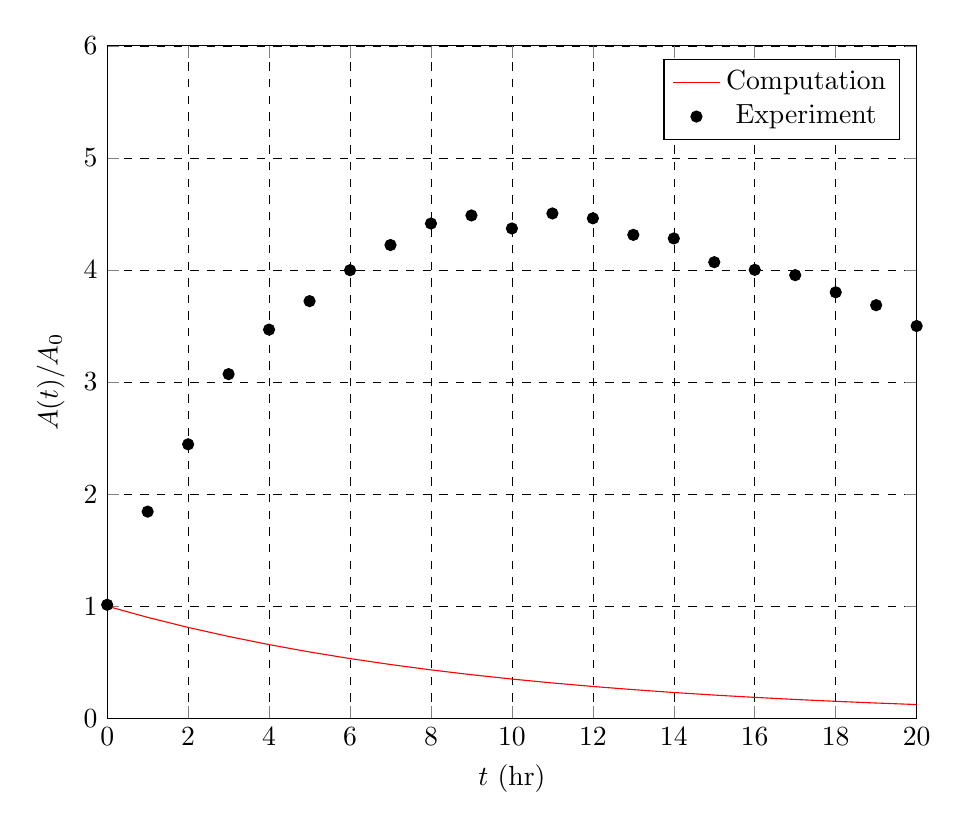
\begin{tikzpicture} \begin{axis}
[scale=1.5,
 xmin=0,    xmax=20,
 ymin=-0, ymax=6,
 grid=major, 
 major grid style={color=black,line width=0.2pt, dashed},
 xlabel=$t$ (hr),
 ylabel=$A(t)/A_0$,
]
%\addplot[
%   black,
%   domain=0:5,
%   samples=201,
%   line width=0.8pt
%]
%{exp(-x)};
%\addlegendentry{analytic}

\addplot[color=red] coordinates {
 ( 0 , 1 ) 
 ( 1 , 0.900324 ) 
 ( 2 , 0.810583 ) 
 ( 3 , 0.729788 ) 
 ( 4 , 0.657045 ) 
 ( 5 , 0.591554 ) 
 ( 6 , 0.53259 ) 
 ( 7 , 0.479504 ) 
 ( 8 , 0.431709 ) 
 ( 9 , 0.388678 ) 
 ( 10 , 0.349936 ) 
 ( 11 , 0.315056 ) 
 ( 12 , 0.283652 ) 
 ( 13 , 0.255379 ) 
 ( 14 , 0.229924 ) 
 ( 15 , 0.207006 ) 
 ( 16 , 0.186372 ) 
 ( 17 , 0.167795 ) 
 ( 18 , 0.15107 ) 
 ( 19 , 0.136012 ) 
 ( 20 , 0.122455 ) 
};
\addlegendentry{Computation}
\addplot[mark=*, only marks] coordinates {
 ( 0 , 1.01259 ) 
 ( 1 , 1.84374 ) 
 ( 2 , 2.44435 ) 
 ( 3 , 3.07065 ) 
 ( 4 , 3.46769 ) 
 ( 5 , 3.72179 ) 
 ( 6 , 3.99806 ) 
 ( 7 , 4.22241 ) 
 ( 8 , 4.41441 ) 
 ( 9 , 4.48648 ) 
 ( 10 , 4.37021 ) 
 ( 11 , 4.50419 ) 
 ( 12 , 4.46095 ) 
 ( 13 , 4.31325 ) 
 ( 14 , 4.28115 ) 
 ( 15 , 4.06937 ) 
 ( 16 , 4.00115 ) 
 ( 17 , 3.9536 ) 
 ( 18 , 3.8006 ) 
 ( 19 , 3.68569 ) 
 ( 20 , 3.49992 ) 
};
\addlegendentry{Experiment}
\end{axis}
\end{tikzpicture}
\caption{Validation of exponential decay model for $^{135}$Xe.}
 \label{Fig:intro_radioactiveDecayValidation_135Xe}
\end{center}
\end{figure}

Next, consider the radioisotope $^{135}$I, which is a common product of nuclear fission and has a half life of about 6.6~hr or a decay constant of $\lambda = 0.105$~hr$^{-1}$. The calculation versus the (simulated) experimental data is shown in Fig.~\ref{Fig:intro_radioactiveDecayValidation_135Xe}. Clearly, the computed activity does not agree with the experimental data at all. In fact, the measured activity increases initially and then decreases. What explains this is that $^{135}$I decays to $^{135}$Xe, which is itself radioactive and has a half life of 9.2 hours and decays to nearly stable $^{135}$Cs. The single decay model being used by the computation does not account for the secondary decays of $^{135}$Xe and cannot therefore adequately reproduce this experimental data. In terms of validation, it can be said that the mathematical model is not suitable for $^{135}$I.

\subsection{Comment on Analytical Models}

While it is rare for an analytical model to be good enough for practical design calculations, this course still covers many of those analytical techniques. The reason for this is while it may be impossible to solve the equations for the actual engineering application directly, most such applications follow some general principles and trends. The analytical methods can provide physical insight into, for example, the general shape of a particular temperature or radiation field, and the expected behavior of how making design changes will impact a system. While sometimes one encounters counterintuitive results, it is more often that when calculations do not follow mathematical intuition from simpler models, there is usually something wrong with the way the software is being used (e.g., errors in input) or there are misunderstandings on the part of the engineer about the physics of the system being analyzed.

